\documentclass[a4paper, 10pt]{article}
\usepackage{graphicx}
\usepackage{amsmath}
\usepackage{hyperref}
\hypersetup{colorlinks=false}

\author{George Zakhour}
\title{{\bf Simulating a two dimensional particle in a square quantum box with
        CUDA}}
\date{\today}

\begin{document}

\maketitle
\newpage
\tableofcontents
\newpage

\section{Background, Motive and Experiment}
The particle in box problem is one of the first problems given to undergraduate
students in a course about quantum mechanics. It showcases how the energy
of particles is quantized and it highlights the probabilistic nature of
quantum mechanics, especially with the idea that the particle is not located in
a fixed position but it has a likelihood of existing at any point in space.\\\\
The particle in a box is an experiment in which a particle is stuck inside a
box and cannot escape. The energy outside this box is $\infty$ while inside it
is $0$. The particle thus moves inside the box of dimensions $L$x$L$.\\\\
Trying to imagine how these probabilities are scattered in the box is hard and one
can't do without a simulation of the physical properties of the particle
(position, energy and momentum).\\\\
In this simulation I try and simulate the "particle in a box" problem to
display the probabilities of the position and the energy of the particle at
each state.

\section{Expected Output}
Searching online, I have found a Youtube video that simulates the particle in a
box\footnote{ Particle in a Box - Youtube {\emph
http://www.youtube.com/watch?v=jevKmFfcaxE}}, but lacks essential information
on the state of the system, for example the dimensions of the box and the
energy levels of the particle at each frame. Although lacking these
essential variables I will base my results on the video.\\

\begin{figure}[hb]
    \centering
        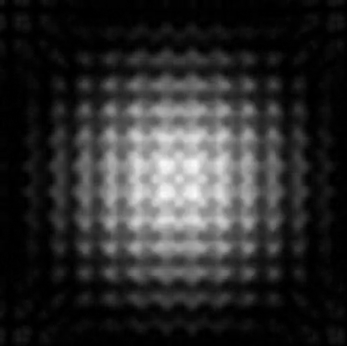
\includegraphics[width=5cm]{graphics/online_simulation.png}
    \caption{A screenshot of a "particle in a box" simulation found on Youtube}
\end{figure}

\newpage

\section{The mathematics of a particle in a box}
    \subsection{In one dimension}
        \subsubsection{Finding the Wave Function from Schrodinger's Equation}
        \label{sec:wave_equation_oned}
        The time dependent Schrodinger equation is given as:
        \begin{equation} \label{eq:time_dependant_equation}
            \left ( \frac{-\hbar^2}{2m} \nabla^2 + V \right ) \Psi(x,t)
            = i\hbar\frac{\partial}{\partial t}\Psi(x, t)   
        \end{equation}
        The time independent Schrodinger equation is given as:
        \begin{equation} \label{eq:time_independent_equation}
            \left ( \frac{-\hbar^2}{2m} \nabla^2 + V \right ) \Phi(x)
            = E \Phi(x)
        \end{equation}
        Where $\Psi$ is the wave equation. In terms of $\Phi$, $\Psi$ is
        denoted as:
        \begin{equation} \label{eq:dep_in_equation}
            \Psi(x, t) = e^{-i(E/\hbar)t}\Phi(x)
        \end{equation}
        Assuming the following is a solution to (\ref{eq:time_independent_equation}):
        \begin{equation} \label{eq:assumed_solution}
            \Phi(x) = A\cos(kx) + B\sin(kx)
        \end{equation}
        And given these two conditions that arise from the experiment:
        $$ \Phi(0) = \Phi(L) = 0 $$
        We plug them in the (\ref{eq:assumed_solution}) and find the following:
        \begin{align}
            \left\{\begin{matrix}
            A & = & 0 \\ 
            k & = & \frac{n}{L}\pi & \text{(n is the energy level)}
            \end{matrix}\right.
        \end{align}
        To find the value of $B$ we need to normalize the equation.\\
        The probability of finding the particle inside $[0; L]$ is $1$ because
        it cannot escape.
        \begin{align}
            \int_{0}^{L} |\Phi|^2 dx &= 1  \\
            B^2\int_{0}^{L} \sin^2\left ( \frac{n}{L}\pi x \right ) dx &= 1
        \end{align}
        And thus $B = \sqrt{\frac{2}{L}}$.\\
        Finally we get the solution to the time independent Schrodinger equation
        \begin{align}
            \Phi(x) = \sqrt{\frac{2}{L}}\sin(\frac{n}{L}\pi x)
        \end{align}

        \subsubsection{Energy at each quantum level $n$}
        \label{sec:energy_oned}
        We note the following
        \begin{align}
            \frac{\partial^2 }{\partial x^2} \Phi = -\left (
            \frac{n\pi}{L}\right )^2 \Phi
        \end{align}
        If we replace the results in (\ref{eq:time_independent_equation}) we find:
        $$ E_n = \frac{\hbar^2 n^2 \pi^2}{ 2 m L^2} $$
        Or simply:
        \begin{align*}
            E_n &= n^2 E_1 \\
            E_1 &= \frac{\hbar^2 \pi^2}{2 m L^2}
        \end{align*}

        \subsubsection{Probability function of the position}
        \label{sec:position_oned}
        The probability of finding the particle between $a$ and $b$ is the following:
        \begin{equation} \label{eq:probability_position}
            \left\{\begin{matrix}
            \int_{a}^{b} |\Phi|^2 dx & \text{if} \; \: a,b \in [0, L] \\ 
            0 & \text{otherwise}
            \end{matrix}\right.
        \end{equation}
        If we wish to find the position inside a box of width $\epsilon$ and
        center $a$ we would integrate between $a-\epsilon/2$ and $a+\epsilon/2$
        where both ends are between $0$ and $L$\\
        The integration will lead to the following:
        $$ P(x) = \frac{\epsilon}{L} + \frac{1}{2n\pi} \left [ 
            \sin\left ( \frac{2n\pi}{L}(a - \epsilon/2)\right ) -
            \sin\left ( \frac{2n\pi}{L}(a + \epsilon/2)\right )
        \right ]$$
        Which can be reduced more to the following form:
        $$ P(x) = \frac{\epsilon}{L} - \frac{1}{n\pi}\sin\left( \frac{n\pi}{L}\epsilon \right)
        \cos\left(\frac{2n\pi}{L}x\right)$$

    \subsection{In two dimensions}
        \subsubsection{The time-independent solution}
        This time we suppose the solution is
        \begin{equation} \label{eq:suppose_twod_solution}
            \Phi(x, y) = X(x)Y(y)
        \end{equation}
        \begin{align*}
            X(x) &= A\cos(k_x x) + B \sin(k_x x) \\
            Y(y) &= C\cos(k_y y) + D \sin(k_y y) \\
        \end{align*}
        Plugging (\ref{eq:suppose_twod_solution}) in (\ref{eq:time_independent_equation})
        and doing similar operations as \emph{~\ref{sec:wave_equation_oned}} we get
        the following solution:
        \begin{equation} \label{eq:twod_solution}
            \Phi(x, y) = \frac{2}{L} \sin\left( \frac{n_x\pi}{L}x\right)
                         \sin\left( \frac{n_y\pi}{L} y\right)
        \end{equation}

        \subsubsection{Energy in two dimensions}
        Doing the same steps as \emph{~\ref{sec:energy_oned}} we find that the energy has
        become:
        \begin{align}
            E_{n_x, n_y} &= \frac{\hbar^2 \pi^2}{2mL^2} (n^2_x + n^2_y)
        \end{align}
        Or simply:
        \begin{align*}
        E_{n_x, n_y} &= (n^2_x + n^2_y) \; E_{1,1} \\
        E_{1,1} &= \frac{\hbar^2 \pi^2}{2mL^2} 
        \end{align*}

        \subsubsection{Probability function of the position}
        Similar to section \emph{~\ref{sec:position_oned}} to find the
        probability of finding the particle inside the box of size
        $\epsilon$x$\epsilon$ we integrate the wave function inside a
        box of center $(x,y)$ and width $\epsilon$.
        $$ P(x, y) = \int^{y+\epsilon/2}_{y-\epsilon/2}\int^{x+\epsilon/2}_{x-\epsilon/2}
          |\Phi(x, y)|^2 dx dy $$
        After evaluating the integral we get the following function:
        \begin{equation} \label{eq:position_twod_equation}
            P(x, y) = \frac{1}{L^2} \; p(x) \; p(y)
        \end{equation}
        $$
        p(\alpha) = \epsilon - \frac{L}{n_\alpha\pi} \cos\left( \frac{2n_\alpha\pi}{L}\alpha \right)
        \sin\left( \frac{n_\alpha\pi}{L} \epsilon\right)
        $$

        \subsection{Generalizing the time-independent solution}
        The equation that we have found so far depends on two quantum numbers
        $n_x$ and $n_y$ and describes the particle for these energy levels only.
        However the final time-dependant equation is a combination of many of these
        equations. The final time-independent equation is:
        \begin{equation} \label{eq:general_position}
            \Phi(x,y) = \sum_{n} c_n \Phi_{n_x, n_y}(x,y)
        \end{equation}
        Where the constant $c_n$ is the square root of the probability of getting
        the equation $\Phi_{n_x, n_y}$ that describes the particle in the box.

        \subsection{Generalizing the probability function}
        Since we have a more general wave function we need to have a more general
        probability function for the position. The new definition is generated from
        integrating $\Phi$ between $a-\epsilon/2$ and $a+\epsilon/2$. The result is:
        $$ P(x, y) = \sum_{n} c^2_n \: P_n(x, y)$$

\newpage

\section{Implementation}
    \subsection{Conventions}
    Some of the conventions adopted through the code are
    \begin{itemize}
        \item words in function and struct names are seperated by an \_ (underscore)
        \item words in variable names are glued together with the first letter
              capitalized. Except in the case of the first character.
        \item functions that start with \_ are helper functions
              and should not be used directly. They may be considered like private
              methods and properties in object-oriented code. No major documentation
              is provided for these functions and the author only uses inline code
              comments to document them
        \item Tiny mathematical and physical constants, such as $\hbar$ are expressed
              as float numbers without their orders. For example $\hbar = 1.054\cdot10^{-34}$
              is defined the following way \texttt{\#define HBAR 1.054 // without e-34}
    \end{itemize}


\newpage
\section{API}
    \subsection{Structs}
        \subsubsection{\texttt{\_wave\_function}}
        This struct is used by the \texttt{particle} struct and describes a wave function
        \begin{itemize}
            \item \texttt{int n} the energy level of the particle described by the wave function
            \item \texttt{float energy} the energy of the particle at that energy level
        \end{itemize}
        \subsubsection{\texttt{particle}}
        This struct represents a particle and have the following elements
        \begin{itemize}
            \item \texttt{float mass} the mass of the particle
            \item \texttt{\_wave\_function* wave} the wave function that describes the state of
                  the particle
        \end{itemize}

    \subsection{Functions}
        \subsubsection{\texttt{create\_particle}}
        This function is used to create a new particle.
        \begin{verbatim}
void create_particle(particle* p, int n, float mass);
        \end{verbatim}
        \begin{itemize}
            \item \texttt{particle* p} the particle to create
            \item \texttt{int n} the energy level of the particle
            \item \texttt{float mass} the mass of the particle
        \end{itemize}
        \subsubsection{\texttt{probability}}
        This function finds the probability of finding the particle in the box of center $(x, y)$
        and of dimensions $\epsilon$x$\epsilon$\\
        The function returns a \texttt{float}; the probability of finding the particle at points (x, y)
        \begin{verbatim}
float probability(particle *p, float x, float y);
        \end{verbatim}
        \begin{itemize}
            \item \texttt{particle* p} the particle to find the probability of
            \item \texttt{float x} the x-coordinate of the center of the box 
            \item \texttt{float y} the y-coordinate of the center of the box
        \end{itemize}

\newpage
\section{Results}

\newpage
\section{Code}
    \subsection{Code}
\begin{verbatim}
\end{verbatim}
    \subsection{License: GNU General Public License}
    Copyright (C) 2013 George Zakhour\\

    This program is free software: you can redistribute it and/or modify it under
    the terms of the GNU General Public License as published by the Free Software
    Foundation, either version 3 of the License, or (at your option) any later
    version.\\

    This program is distributed in the hope that it will be useful, but WITHOUT ANY
    WARRANTY; without even the implied warranty of MERCHANTABILITY or FITNESS FOR A
    PARTICULAR PURPOSE. See the GNU General Public License for more details.\\

    You should have received a copy of the GNU General Public License along with
    this program. If not, see http://www.gnu.org/licenses/.\\


\end{document}
